%=========================================================================%
%                                 bar.tex                                 %
%                                                                         %
% Author: Nic H.                                                          %
% Date: 2016-Mar-17                                                       %
%=========================================================================%

\documentclass{beamer}

\usepackage{standalone}
\usepackage{tikz}
\usepackage{pgfplots}

\renewcommand\familydefault{\sfdefault}

\title{Bar}
\author{Nic H.}
\date{\today}

\begin{document}

\begin{frame}
\maketitle
\end{frame}

\begin{frame}
this is a figure.

\begin{figure}[b]
    % Bar charts
% Author: Stefan Kottwitz
% https://www.packtpub.com/hardware-and-creative/latex-cookbook
\documentclass[border=10pt]{standalone}
\usepackage{pgfplots}
\begin{document}
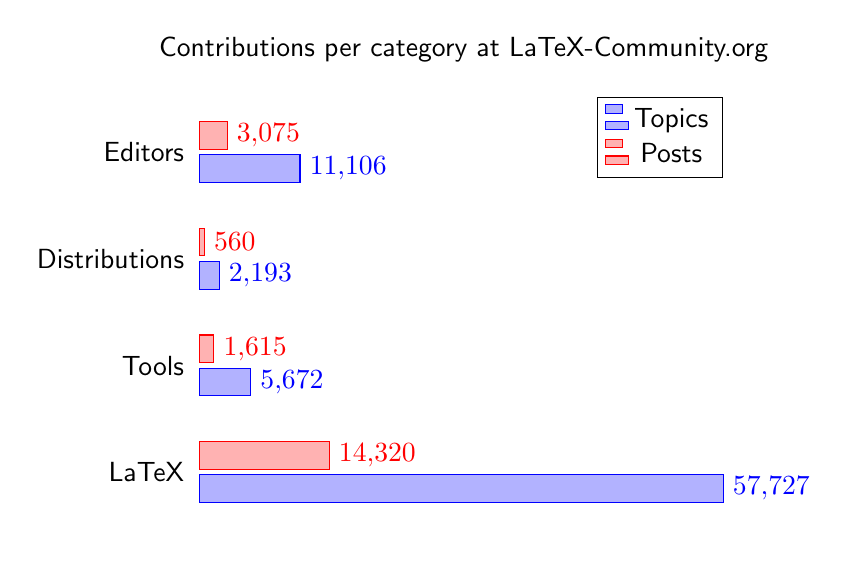
\begin{tikzpicture}
    \begin{axis}[title  = Contributions per category
            at LaTeX-Community.org,
            xbar,
            y axis line style = { opacity = 0 },
            axis x line       = none,
            tickwidth         = 0pt,
            enlarge y limits  = 0.2,
            enlarge x limits  = 0.02,
            symbolic y coords = {LaTeX, Tools, Distributions, Editors},
            nodes near coords,
        ]
        \addplot coordinates { (57727,LaTeX)         (5672,Tools)
        (2193,Distributions)  (11106,Editors) };
        \addplot coordinates { (14320,LaTeX)         (1615,Tools)
        (560,Distributions)   (3075,Editors)  };
        \legend{Topics, Posts}
    \end{axis}
\end{tikzpicture}
\end{document}

    \caption{i am a cpation}
    \label{fig1}
\end{figure}

as we see in figure~\ref{fig1}.
\end{frame}

\begin{frame}
    \begin{figure}
        
\documentclass[beamer=true]{standalone}
\usepackage{tikz}
\begin{document}
\begin{standaloneframe}
    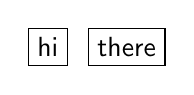
\begin{tikzpicture}
        \node[draw] (h) {hi};
        \node<2->[draw,right of= h] (y) {there};
    \end{tikzpicture}
\end{standaloneframe}
\end{document}

        \caption{another caption}
    \end{figure}
    \begin{itemize}
        \item a
        \item b
    \end{itemize}
\end{frame}

\end{document}
